\section{Results}
\label{sec:results}

\subsection{Learning curves}

\begin{figure}[t]
  \centering
  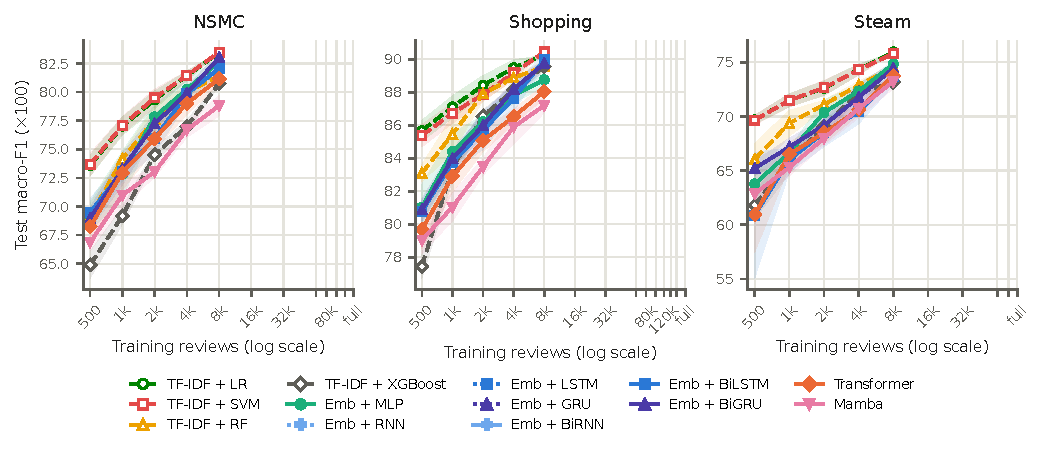
\includegraphics[width=\linewidth]{figures/fig2_learning_curves.pdf}
  \caption{Learning curves: test macro-F1 versus training size (log scale) for all
  thirteen methods; shaded bands are $\pm1$ standard deviation over \nSeeds{} seeds
  (sample std, ddof\,=\,1). Dashed lines with hollow markers are TF-IDF methods;
  solid lines with filled markers are neural methods. The dotted vertical line marks
  the crossover threshold when one exists.}
  \label{fig:curves}
\end{figure}

\begin{table}[t]
  \centering
  \caption{Test macro-F1 ($\times100$) across training sizes. \pmnote{} Bold: best
  mean in the column within each dataset. $^{\dagger}$/$^{\ddagger}$: best TF-IDF /
  best neural method at that size, selected by validation macro-F1 (the pair used for
  the crossover).}
  \label{tab:f1}
  % AUTO-GENERATED by ksent.analysis.make_tables (do not edit by hand).
\begin{adjustbox}{max width=\linewidth}
\begin{tabular}{lrrrrrrrrrrrrrr}
\toprule
Method & $n$=500 & $n$=1{,}000 & $n$=2{,}000 & $n$=4{,}000 & $n$=8{,}000 & $n$=16{,}000 & $n$=32{,}000 & $n$=64{,}000 & $n$=80{,}000 & $n$=100{,}000 & $n$=120{,}000 & $n$=140{,}000 & $n$=160{,}000 & full \\
\midrule
\multicolumn{15}{l}{\textit{NSMC} (full = 143{,}640)} \\
TF-IDF + LR & 73.59{\scriptsize$\pm$0.89} & 77.03{\scriptsize$\pm$0.77} & 79.32{\scriptsize$\pm$0.76} & 81.43{\scriptsize$\pm$0.40}$^{\dagger}$ & 83.45{\scriptsize$\pm$0.00} & -- & -- & -- & -- & -- & -- &  &  & -- \\
TF-IDF + SVM & \textbf{73.67}{\scriptsize$\pm$0.95}$^{\dagger}$ & \textbf{77.10}{\scriptsize$\pm$0.75}$^{\dagger}$ & \textbf{79.49}{\scriptsize$\pm$0.75}$^{\dagger}$ & \textbf{81.45}{\scriptsize$\pm$0.39} & \textbf{83.50}{\scriptsize$\pm$0.00}$^{\dagger}$ & -- & -- & -- & -- & -- & -- &  &  & -- \\
TF-IDF + RF & 69.13{\scriptsize$\pm$1.11} & 74.15{\scriptsize$\pm$0.53} & 77.63{\scriptsize$\pm$1.06} & 79.98{\scriptsize$\pm$0.66} & 81.43{\scriptsize$\pm$0.23} & -- & -- & -- & -- & -- & -- &  &  & -- \\
TF-IDF + XGBoost & 64.90{\scriptsize$\pm$1.15} & 69.19{\scriptsize$\pm$0.73} & 74.54{\scriptsize$\pm$0.50} & 77.01{\scriptsize$\pm$0.55} & 80.76{\scriptsize$\pm$0.14} & -- & -- & -- & -- & -- & -- &  &  & -- \\
\cmidrule(lr){1-15}
Emb + MLP & 69.16{\scriptsize$\pm$1.29} & 72.84{\scriptsize$\pm$1.99} & 77.84{\scriptsize$\pm$1.04}$^{\ddagger}$ & 80.24{\scriptsize$\pm$0.78}$^{\ddagger}$ & 82.65{\scriptsize$\pm$0.40} & -- & -- & -- & -- & -- & -- &  &  & -- \\
Emb + RNN & -- & -- & -- & -- & -- & -- & -- & -- & -- & -- & -- &  &  & -- \\
Emb + LSTM & -- & -- & -- & -- & -- & -- & -- & -- & -- & -- & -- &  &  & -- \\
Emb + GRU & -- & -- & -- & -- & -- & -- & -- & -- & -- & -- & -- &  &  & -- \\
Emb + BiRNN & -- & -- & -- & -- & -- & -- & -- & -- & -- & -- & -- &  &  & -- \\
Emb + BiLSTM & 69.50{\scriptsize$\pm$1.22} & 73.06{\scriptsize$\pm$0.83} & 75.96{\scriptsize$\pm$1.32} & 79.84{\scriptsize$\pm$0.70} & 82.08{\scriptsize$\pm$0.64} & -- & -- & -- & -- & -- & -- &  &  & -- \\
Emb + BiGRU & 68.96{\scriptsize$\pm$0.96}$^{\ddagger}$ & 73.26{\scriptsize$\pm$1.35}$^{\ddagger}$ & 77.23{\scriptsize$\pm$0.86} & 79.89{\scriptsize$\pm$0.51} & 83.02{\scriptsize$\pm$0.49}$^{\ddagger}$ & -- & -- & -- & -- & -- & -- &  &  & -- \\
Transformer & 68.25{\scriptsize$\pm$1.12} & 72.96{\scriptsize$\pm$1.48} & 75.92{\scriptsize$\pm$0.90} & 79.02{\scriptsize$\pm$0.96} & 81.16{\scriptsize$\pm$0.44} & -- & -- & -- & -- & -- & -- &  &  & -- \\
Mamba & 66.88{\scriptsize$\pm$0.73} & 71.00{\scriptsize$\pm$1.02} & 73.03{\scriptsize$\pm$0.44} & 76.71{\scriptsize$\pm$0.66} & 78.81{\scriptsize$\pm$0.87} & -- & -- & -- & -- & -- & -- &  &  & -- \\
\midrule
\multicolumn{15}{l}{\textit{Shopping} (full = 195{,}881)} \\
TF-IDF + LR & \textbf{85.67}{\scriptsize$\pm$0.62}$^{\dagger}$ & \textbf{87.11}{\scriptsize$\pm$0.66}$^{\dagger}$ & \textbf{88.42}{\scriptsize$\pm$0.59}$^{\dagger}$ & \textbf{89.49}{\scriptsize$\pm$0.47}$^{\dagger}$ & 90.25{\scriptsize$\pm$0.00} & -- & -- & -- & -- & -- & -- & -- & -- & -- \\
TF-IDF + SVM & 85.37{\scriptsize$\pm$0.67} & 86.73{\scriptsize$\pm$0.61} & 87.87{\scriptsize$\pm$0.41} & 89.17{\scriptsize$\pm$0.37} & \textbf{90.45}{\scriptsize$\pm$0.00}$^{\dagger}$ & -- & -- & -- & -- & -- & -- & -- & -- & -- \\
TF-IDF + RF & 83.09{\scriptsize$\pm$0.51} & 85.46{\scriptsize$\pm$1.10} & 87.90{\scriptsize$\pm$0.39} & 88.87{\scriptsize$\pm$0.13} & 89.55{\scriptsize$\pm$0.33} & -- & -- & -- & -- & -- & -- & -- & -- & -- \\
TF-IDF + XGBoost & 77.44{\scriptsize$\pm$0.71} & 83.42{\scriptsize$\pm$0.75} & 86.56{\scriptsize$\pm$0.36} & 88.13{\scriptsize$\pm$0.31} & 89.57{\scriptsize$\pm$0.22} & -- & -- & -- & -- & -- & -- & -- & -- & -- \\
\cmidrule(lr){1-15}
Emb + MLP & 81.04{\scriptsize$\pm$1.39}$^{\ddagger}$ & 84.40{\scriptsize$\pm$1.09}$^{\ddagger}$ & 86.21{\scriptsize$\pm$0.39}$^{\ddagger}$ & 87.83{\scriptsize$\pm$0.47} & 88.76{\scriptsize$\pm$0.39} & -- & -- & -- & -- & -- & -- & -- & -- & -- \\
Emb + RNN & -- & -- & -- & -- & -- & -- & -- & -- & -- & -- & -- & -- & -- & -- \\
Emb + LSTM & -- & -- & -- & -- & -- & -- & -- & -- & -- & -- & -- & -- & -- & -- \\
Emb + GRU & -- & -- & -- & -- & -- & -- & -- & -- & -- & -- & -- & -- & -- & -- \\
Emb + BiRNN & -- & -- & -- & -- & -- & -- & -- & -- & -- & -- & -- & -- & -- & -- \\
Emb + BiLSTM & 80.77{\scriptsize$\pm$0.67} & 83.75{\scriptsize$\pm$0.49} & 85.69{\scriptsize$\pm$1.16} & 87.64{\scriptsize$\pm$0.77} & 89.96{\scriptsize$\pm$0.39}$^{\ddagger}$ & -- & -- & -- & -- & -- & -- & -- & -- & -- \\
Emb + BiGRU & 80.87{\scriptsize$\pm$0.66} & 83.99{\scriptsize$\pm$0.56} & 85.98{\scriptsize$\pm$0.63} & 88.19{\scriptsize$\pm$0.51}$^{\ddagger}$ & 89.74{\scriptsize$\pm$0.20} & -- & -- & -- & -- & -- & -- & -- & -- & -- \\
Transformer & 79.69{\scriptsize$\pm$1.17} & 82.90{\scriptsize$\pm$0.95} & 85.08{\scriptsize$\pm$0.67} & 86.52{\scriptsize$\pm$0.44} & 88.04{\scriptsize$\pm$0.41} & -- & -- & -- & -- & -- & -- & -- & -- & -- \\
Mamba & 79.04{\scriptsize$\pm$0.81} & 81.04{\scriptsize$\pm$0.84} & 83.48{\scriptsize$\pm$0.50} & 85.89{\scriptsize$\pm$1.03} & 87.20{\scriptsize$\pm$0.44} & -- & -- & -- & -- & -- & -- & -- & -- & -- \\
\midrule
\multicolumn{15}{l}{\textit{Steam} (full = 95{,}774)} \\
TF-IDF + LR & \textbf{69.68}{\scriptsize$\pm$0.39}$^{\dagger}$ & \textbf{71.49}{\scriptsize$\pm$0.59} & 72.60{\scriptsize$\pm$0.66}$^{\dagger}$ & \textbf{74.33}{\scriptsize$\pm$0.48}$^{\dagger}$ & \textbf{75.95}{\scriptsize$\pm$0.00}$^{\dagger}$ & -- & -- & -- & -- &  &  &  &  & -- \\
TF-IDF + SVM & 69.66{\scriptsize$\pm$0.44} & 71.48{\scriptsize$\pm$0.58}$^{\dagger}$ & \textbf{72.64}{\scriptsize$\pm$0.67} & 74.30{\scriptsize$\pm$0.46} & 75.80{\scriptsize$\pm$0.00} & -- & -- & -- & -- &  &  &  &  & -- \\
TF-IDF + RF & 66.03{\scriptsize$\pm$1.49} & 69.37{\scriptsize$\pm$1.18} & 71.09{\scriptsize$\pm$0.40} & 72.89{\scriptsize$\pm$0.34} & 74.49{\scriptsize$\pm$0.24} & -- & -- & -- & -- &  &  &  &  & -- \\
TF-IDF + XGBoost & 61.78{\scriptsize$\pm$1.19} & 65.98{\scriptsize$\pm$1.27} & 69.04{\scriptsize$\pm$0.73} & 72.20{\scriptsize$\pm$0.53} & 73.15{\scriptsize$\pm$0.18} & -- & -- & -- & -- &  &  &  &  & -- \\
\cmidrule(lr){1-15}
Emb + MLP & 63.77{\scriptsize$\pm$1.31} & 66.64{\scriptsize$\pm$0.44} & 70.36{\scriptsize$\pm$1.16} & 72.34{\scriptsize$\pm$0.61}$^{\ddagger}$ & 74.83{\scriptsize$\pm$0.24}$^{\ddagger}$ & -- & -- & -- & -- &  &  &  &  & -- \\
Emb + RNN & -- & -- & -- & -- & -- & -- & -- & -- & -- &  &  &  &  & -- \\
Emb + LSTM & -- & -- & -- & -- & -- & -- & -- & -- & -- &  &  &  &  & -- \\
Emb + GRU & -- & -- & -- & -- & -- & -- & -- & -- & -- &  &  &  &  & -- \\
Emb + BiRNN & -- & -- & -- & -- & -- & -- & -- & -- & -- &  &  &  &  & -- \\
Emb + BiLSTM & 60.87{\scriptsize$\pm$5.79} & 66.00{\scriptsize$\pm$1.10} & 68.52{\scriptsize$\pm$1.30} & 70.42{\scriptsize$\pm$1.08} & 73.66{\scriptsize$\pm$0.76} & -- & -- & -- & -- &  &  &  &  & -- \\
Emb + BiGRU & 65.20{\scriptsize$\pm$0.67}$^{\ddagger}$ & 67.18{\scriptsize$\pm$0.80}$^{\ddagger}$ & 69.17{\scriptsize$\pm$0.60}$^{\ddagger}$ & 71.76{\scriptsize$\pm$1.24} & 74.43{\scriptsize$\pm$0.52} & -- & -- & -- & -- &  &  &  &  & -- \\
Transformer & 60.95{\scriptsize$\pm$3.49} & 66.51{\scriptsize$\pm$1.08} & 68.48{\scriptsize$\pm$0.98} & 70.63{\scriptsize$\pm$0.46} & 73.75{\scriptsize$\pm$0.40} & -- & -- & -- & -- &  &  &  &  & -- \\
Mamba & 62.87{\scriptsize$\pm$0.76} & 65.29{\scriptsize$\pm$0.77} & 67.98{\scriptsize$\pm$0.64} & 70.73{\scriptsize$\pm$0.83} & 73.22{\scriptsize$\pm$0.63} & -- & -- & -- & -- &  &  &  &  & -- \\
\bottomrule
\end{tabular}
\end{adjustbox}

\end{table}

\Cref{fig:curves} and \cref{tab:f1} show test macro-F1 for every method and size.
At $n=8{,}000$ the best method is \bestMethodNSMC{} on NSMC
(\macroFOneBestNSMC), \bestMethodShopping{} on Shopping (\macroFOneBestShopping)
and \bestMethodSteam{} on Steam (\macroFOneBestSteam).
TF-IDF leads clearly at the smallest size: at $n=500$ the best neural method trails the
best TF-IDF method (both Kiwi-tokenised, selected on validation) by \ablationGapSmallNSMC{}
(NSMC), \ablationGapSmallShopping{} (Shopping) and \ablationGapSmallSteam{} (Steam) points.
Neural curves rise faster, so the gap narrows with data, but the curves of the two family
winners never cross on any dataset: at $n=8{,}000$ the gap is still \gapNSMC,
\gapShopping{} and \gapSteam{} points. One plausible reason for the slow neural start is
vocabulary coverage. With the neural vocabulary built from the training subset
(min.\ frequency 2), \oovSmallNSMC{} (NSMC), \oovSmallShopping{} (Shopping) and
\oovSmallSteam{} (Steam) of test tokens are out of vocabulary at $n=500$, against
\oovLargeNSMC, \oovLargeShopping{} and \oovLargeSteam{} at $n=8{,}000$ (\cref{fig:oov}).
Embeddings trained from scratch on a few thousand reviews have little signal for rare
morphemes, whereas sublinear TF-IDF with a linear model needs no learned representation.
Among the TF-IDF methods, linear models (LR, SVM) dominate RF and XGBoost at every size.
Among the neural methods, the simple embedding models (MLP, GRU, LSTM) are ahead of the
Transformer and Mamba (\cref{sec:discussion}). No method has saturated by $n=8{,}000$
(\cref{sec:marginal}).

\subsection{Crossover thresholds}

\begin{sidewaystable}
  \centering
  \caption{Crossover threshold and cost by dataset. Winners are chosen per size by
  validation macro-F1; the threshold is the smallest size where the mean paired test
  macro-F1 gap (neural $-$ TF-IDF, points) is at least \crossoverMargin. Gap and costs
  are reported at the threshold, or at $n=8{,}000$ when there is no crossover. \pmnote{}
  ``Pareto'': the neural winner is not dominated by the TF-IDF winner on (macro-F1,
  CPU latency, fit time, peak RAM).}
  \label{tab:crossover}
  % AUTO-GENERATED by ksent.analysis.make_tables (do not edit by hand).
\begin{adjustbox}{max width=\linewidth}
\begin{tabular}{lllrrrrrrrrc}
\toprule
Dataset & Best TF-IDF & Best neural & Threshold & Gap (pts) & \multicolumn{2}{c}{Fit e2e (s)} & \multicolumn{2}{c}{CPU e2e latency (ms)} & \multicolumn{2}{c}{Peak RAM (MB)} & Pareto \\
\cmidrule(lr){6-7}\cmidrule(lr){8-9}\cmidrule(lr){10-11}
 & & & & & TF-IDF & Neural & TF-IDF & Neural & TF-IDF & Neural & \\
\midrule
NSMC & TF-IDF + SVM & Emb + BiGRU & none $\le$ full$^{*}$ & -0.48{\scriptsize$\pm$0.49} & 0.898{\scriptsize$\pm$0.077} & 48.8{\scriptsize$\pm$10.1} & 1.04{\scriptsize$\pm$0.06} & 1.21{\scriptsize$\pm$0.01} & 1,445{\scriptsize$\pm$7} & 2,375{\scriptsize$\pm$4} & no \\
Shopping & TF-IDF + SVM & Emb + BiLSTM & none $\le$ full$^{*}$ & -0.49{\scriptsize$\pm$0.39} & 0.997{\scriptsize$\pm$0.089} & 61.1{\scriptsize$\pm$10.6} & 1.04{\scriptsize$\pm$0.07} & 1.50{\scriptsize$\pm$0.02} & 1,453{\scriptsize$\pm$16} & 2,429{\scriptsize$\pm$10} & no \\
Steam & TF-IDF + LR & Emb + MLP & none $\le$ full$^{*}$ & -1.12{\scriptsize$\pm$0.24} & 1.28{\scriptsize$\pm$0.13} & 14.5{\scriptsize$\pm$4.7} & 1.16{\scriptsize$\pm$0.05} & 0.826{\scriptsize$\pm$0.327} & 1,461{\scriptsize$\pm$10} & 2,282{\scriptsize$\pm$10} & yes \\
\bottomrule
\end{tabular}
\end{adjustbox}

\end{sidewaystable}

\Cref{tab:crossover} answers the research question. The crossover threshold is
\crossoverNSMC{} for NSMC (\bestNeuralNSMC{} vs \bestTfidfNSMC, gap \gapNSMC{} points),
\crossoverShopping{} for Shopping (\bestNeuralShopping{} vs \bestTfidfShopping, gap
\gapShopping) and \crossoverSteam{} for Steam (\bestNeuralSteam{} vs \bestTfidfSteam,
gap \gapSteam). Selecting the winners by test instead of validation macro-F1 gives
thresholds of \crossoverTestSelNSMC, \crossoverTestSelShopping{} and
\crossoverTestSelSteam{} (\cref{tab:a4}). The sensitivity check does not change the conclusion. At $n=8{,}000$ validation and test
selection pick the same pair of winners on every dataset. At smaller sizes they sometimes
pick a different pair, but every gap is negative under both rules, so no gap reaches
\crossoverMargin{} point at any size. The research question therefore has the same answer in all three domains:
\emph{no observed crossover up to 8{,}000 reviews}.

\subsection{Quality and cost at 8,000 reviews}

\begin{table}[t]
  \centering
  \caption{Predictive quality at $n=8{,}000$ ($\times100$; from the parallel quality runs).
  \pmnote{} Bold: best per column within a dataset.}
  \label{tab:quality8k}
  % AUTO-GENERATED by ksent.analysis.make_tables (do not edit by hand).
\begin{adjustbox}{max width=\linewidth}
\begin{tabular}{lrrrr}
\toprule
Method & Macro-F1 & Accuracy & Macro-P & Macro-R \\
\midrule
\multicolumn{5}{l}{\textit{NSMC}} \\
TF-IDF + LR & -- & -- & -- & -- \\
TF-IDF + SVM & -- & -- & -- & -- \\
TF-IDF + RF & -- & -- & -- & -- \\
TF-IDF + XGBoost & -- & -- & -- & -- \\
\cmidrule(lr){1-5}
Emb + MLP & -- & -- & -- & -- \\
Emb + LSTM & -- & -- & -- & -- \\
Emb + GRU & -- & -- & -- & -- \\
Transformer & -- & -- & -- & -- \\
Mamba & -- & -- & -- & -- \\
\midrule
\multicolumn{5}{l}{\textit{Shopping}} \\
TF-IDF + LR & -- & -- & -- & -- \\
TF-IDF + SVM & -- & -- & -- & -- \\
TF-IDF + RF & -- & -- & -- & -- \\
TF-IDF + XGBoost & -- & -- & -- & -- \\
\cmidrule(lr){1-5}
Emb + MLP & -- & -- & -- & -- \\
Emb + LSTM & -- & -- & -- & -- \\
Emb + GRU & -- & -- & -- & -- \\
Transformer & -- & -- & -- & -- \\
Mamba & -- & -- & -- & -- \\
\midrule
\multicolumn{5}{l}{\textit{Steam}} \\
TF-IDF + LR & -- & -- & -- & -- \\
TF-IDF + SVM & -- & -- & -- & -- \\
TF-IDF + RF & -- & -- & -- & -- \\
TF-IDF + XGBoost & -- & -- & -- & -- \\
\cmidrule(lr){1-5}
Emb + MLP & -- & -- & -- & -- \\
Emb + LSTM & -- & -- & -- & -- \\
Emb + GRU & -- & -- & -- & -- \\
Transformer & -- & -- & -- & -- \\
Mamba & -- & -- & -- & -- \\
\bottomrule
\end{tabular}
\end{adjustbox}

\end{table}

\begin{sidewaystable}
  \centering
  \caption{Computational cost at $n=8{,}000$. \pmnote{} Fit times in seconds (end-to-end
  includes tokenisation and vectoriser/vocabulary construction); latency is the median
  per-review time at batch size 1 in milliseconds; ``Tune'' is the total fit time of the ten
  tuning runs (single seed); RAM is the peak resident memory of the run's process. Bold:
  lowest cost per column within a dataset. Hardware: \cpuModel{} with \nThreads{} threads
  (CPU columns) and \gpuModel{} (accelerator columns); precision \precisionUsed. Every cost
  comes from exclusive cost runs (one job at a time on an otherwise idle machine), whose
  predictions were identical to the parallel quality runs that supply all predictive
  metrics (\cref{tab:quality8k}).}
  \label{tab:cost}
  % AUTO-GENERATED by ksent.analysis.make_tables (do not edit by hand).
\begin{adjustbox}{max width=\linewidth}
\begin{tabular}{lrrrrrrrrr}
\toprule
Method & Fit e2e (s) & Fit clf.\ (s) & Tune (s) & CPU e2e (ms) & CPU clf.\ (ms) & Accel.\ e2e (ms) & RAM (MB) & Accel.\ mem (MB) & Size (MB) \\
\midrule
\multicolumn{10}{l}{\textit{NSMC}} \\
TF-IDF + LR & -- & -- & -- & -- & -- & n/a & -- & n/a & -- \\
TF-IDF + SVM & -- & -- & -- & -- & -- & n/a & -- & n/a & -- \\
TF-IDF + RF & -- & -- & -- & -- & -- & n/a & -- & n/a & -- \\
TF-IDF + XGBoost & -- & -- & -- & -- & -- & n/a & -- & n/a & -- \\
\cmidrule(lr){1-10}
Emb + MLP & -- & -- & -- & -- & -- & -- & -- & -- & -- \\
Emb + LSTM & -- & -- & -- & -- & -- & -- & -- & -- & -- \\
Emb + GRU & -- & -- & -- & -- & -- & -- & -- & -- & -- \\
Transformer & -- & -- & -- & -- & -- & -- & -- & -- & -- \\
Mamba & -- & -- & -- & -- & -- & -- & -- & -- & -- \\
\midrule
\multicolumn{10}{l}{\textit{Shopping}} \\
TF-IDF + LR & -- & -- & -- & -- & -- & n/a & -- & n/a & -- \\
TF-IDF + SVM & -- & -- & -- & -- & -- & n/a & -- & n/a & -- \\
TF-IDF + RF & -- & -- & -- & -- & -- & n/a & -- & n/a & -- \\
TF-IDF + XGBoost & -- & -- & -- & -- & -- & n/a & -- & n/a & -- \\
\cmidrule(lr){1-10}
Emb + MLP & -- & -- & -- & -- & -- & -- & -- & -- & -- \\
Emb + LSTM & -- & -- & -- & -- & -- & -- & -- & -- & -- \\
Emb + GRU & -- & -- & -- & -- & -- & -- & -- & -- & -- \\
Transformer & -- & -- & -- & -- & -- & -- & -- & -- & -- \\
Mamba & -- & -- & -- & -- & -- & -- & -- & -- & -- \\
\midrule
\multicolumn{10}{l}{\textit{Steam}} \\
TF-IDF + LR & -- & -- & -- & -- & -- & n/a & -- & n/a & -- \\
TF-IDF + SVM & -- & -- & -- & -- & -- & n/a & -- & n/a & -- \\
TF-IDF + RF & -- & -- & -- & -- & -- & n/a & -- & n/a & -- \\
TF-IDF + XGBoost & -- & -- & -- & -- & -- & n/a & -- & n/a & -- \\
\cmidrule(lr){1-10}
Emb + MLP & -- & -- & -- & -- & -- & -- & -- & -- & -- \\
Emb + LSTM & -- & -- & -- & -- & -- & -- & -- & -- & -- \\
Emb + GRU & -- & -- & -- & -- & -- & -- & -- & -- & -- \\
Transformer & -- & -- & -- & -- & -- & -- & -- & -- & -- \\
Mamba & -- & -- & -- & -- & -- & -- & -- & -- & -- \\
\bottomrule
\end{tabular}
\end{adjustbox}

\end{sidewaystable}

\begin{figure}[t]
  \centering
  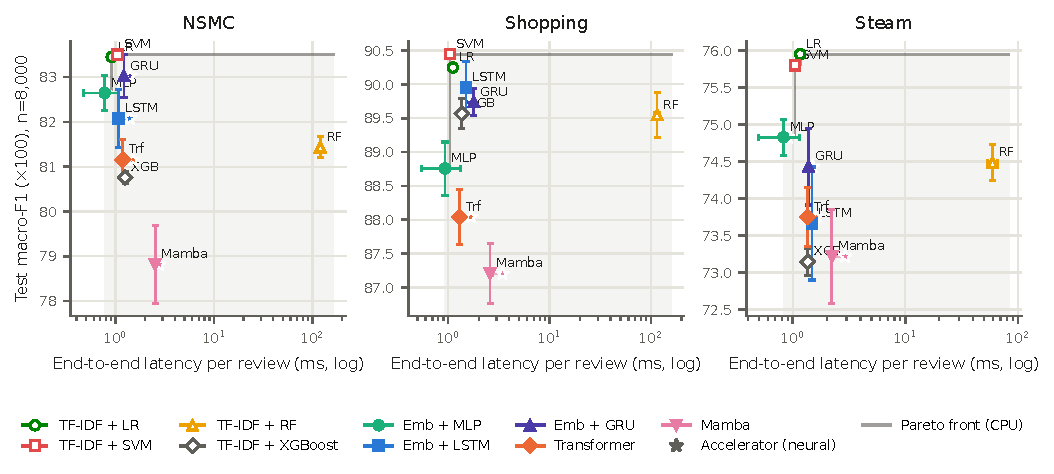
\includegraphics[width=\linewidth]{figures/fig3_quality_vs_cost.pdf}
  \caption{Quality versus inference cost at $n=8{,}000$: test macro-F1 against
  end-to-end CPU latency per review (log scale), error bars $\pm1$ std over \nSeeds{}
  seeds (sample std). Stars connected to neural points show the same model's latency on
  the accelerator (\accelDevice). The grey step line and shaded region mark the CPU Pareto front.}
  \label{fig:cost}
\end{figure}

\Cref{tab:quality8k,tab:cost} and \cref{fig:cost} compare all methods at the largest size.
At the crossover (or at 8{,}000), the neural winner's CPU latency per review is \latencyRatioNSMC{} (NSMC),
\latencyRatioShopping{} (Shopping) and \latencyRatioSteam{} (Steam) that of the TF-IDF
winner, and takes \fitRatioNSMC, \fitRatioShopping{} and
\fitRatioSteam{} longer to fit. It is Pareto-efficient on NSMC: \paretoNSMC;
Shopping: \paretoShopping; Steam: \paretoSteam.
Because there is no crossover, the comparison is made at $n=8{,}000$, where the neural
winner is still \emph{less} accurate. Training is where the two families differ most:
the neural winner needs \fitRatioNSMC, \fitRatioShopping{} and \fitRatioSteam{} the
end-to-end fit time of the TF-IDF winner, and its process peaks at \ramRatioNSMC,
\ramRatioShopping{} and \ramRatioSteam{} the host RAM (the latter mostly reflects the
PyTorch runtime, not the model). Batch-size-1 CPU latency, in contrast, is about one
millisecond for both families (TF-IDF winner \tfidfLatencyNSMC/\tfidfLatencyShopping/\tfidfLatencySteam{} ms,
neural winner \neuralLatencyNSMC/\neuralLatencyShopping/\neuralLatencySteam{} ms on
NSMC/Shopping/Steam). The accelerator does not help at this batch size: the neural winner
takes \neuralAccLatencyNSMC/\neuralAccLatencyShopping/\neuralAccLatencySteam{} ms per
review on the GPU, because kernel launch and host--device transfer dominate a single short
review. The Steam neural winner (Emb\,+\,MLP) is formally Pareto-efficient only because
its mean-pooling network is faster per review than TF-IDF\,+\,LR on the CPU. It is still
\gapSteam{} points less accurate, takes longer to fit and uses more memory, so this is not a
practical argument for switching. Random Forest is the one method whose inference cost
stands out: hundreds of deep trees make it by far the slowest per review and, on Shopping,
by far the largest artefact (\cref{tab:cost}).

\subsection{Class-specific errors}

\begin{figure}[t]
  \centering
  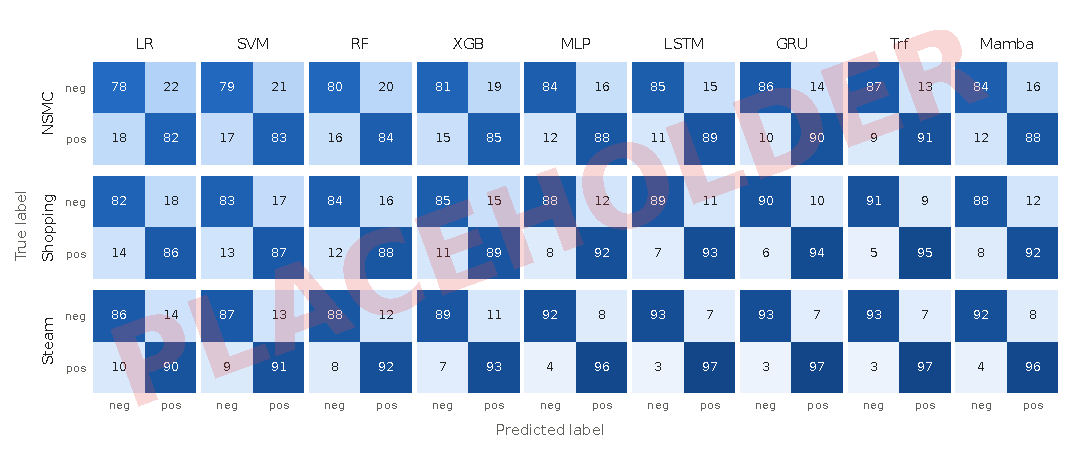
\includegraphics[width=\linewidth]{figures/fig4_confusion.pdf}
  \caption{Confusion matrices at $n=8{,}000$ (rows: true label, columns: predicted),
  counts summed over the \nSeeds{} runs and then row-normalised; cells show
  percentages.}
  \label{fig:confusion}
\end{figure}

\Cref{fig:confusion} shows where the errors fall. On NSMC both winners err at similar
rates on the two classes (TF-IDF: \fprTfidfNSMC{} of negatives predicted positive,
\fnrTfidfNSMC{} of positives predicted negative; neural: \fprNeuralNSMC{} and
\fnrNeuralNSMC). On Shopping the families err in opposite directions: TF-IDF misses more
positives (\fnrTfidfShopping{} vs \fprTfidfShopping), whereas the neural winner
mislabels more negatives (\fprNeuralShopping{} vs \fnrNeuralShopping). This
complementarity suggests that an ensemble could help, which we did not test. Steam is the
hardest domain for both classes and both families: about a quarter of the reviews in
each class are misclassified (TF-IDF \fprTfidfSteam/\fnrTfidfSteam, neural
\fprNeuralSteam/\fnrNeuralSteam), with positives slightly harder. This is consistent with
recommendation flags being a noisy proxy for the sentiment of the text (\cref{sec:limitations}).

\subsection{Marginal value of labels}
\label{sec:marginal}
Doubling the data from 500 to 1{,}000 reviews improves the best 8{,}000-review method by
\gainFirstNSMC, \gainFirstShopping{} and \gainFirstSteam{} points on NSMC, Shopping and
Steam, whereas the last doubling (4{,}000 $\to$ 8{,}000) adds \gainLastNSMC,
\gainLastShopping{} and \gainLastSteam{} points (all gains in \cref{tab:a3}).
None of the curves has flattened. The best TF-IDF method still gains \gainLastNSMC,
\gainLastShopping{} and \gainLastSteam{} points from the last doubling, and the neural
winner gains more (\gainLastNeuralNSMC, \gainLastNeuralShopping{} and
\gainLastNeuralSteam). More labels therefore still pay off for both families, and they
pay off slightly more for neural models. If that trend continued, a crossover beyond
$8{,}000$ reviews would be plausible, but our data cannot show it (\cref{sec:limitations}).
